% D06-001. PDR-05, раздел 8.
\section{Экспертный эталон и проверка его воспроизводимости}
\label{sec:ch5_expert_reference}
\conceptsource{Статья 5, раздел 8. Целевой отбор, раздельная
разметка применимости/направления, повтор одного эксперта
и переходные интервалы. Числа относятся к описанному снимку.}

\subsection{От массового сравнения к ручному разбору}
\conceptsource{Статья 5, трёхмерный стратифицированный отбор.
Сохранены сложность, редкость режима и качество измерений.}

Массовая обработка позволяет сосредоточить экспертный
труд на информативной части архива.
В отборе совместно учитываются сложность решения,
редкость физического режима и качество измерений.
К сложным относятся устойчивые разногласия органов,
работа около уставки и частые переключения.
Редкость описывается несимметрией, кратностью тока
и нетипичным сочетанием электрических величин.
Отдельную группу образуют прогрузки и дефекты сигналов.

(Примечание автора: Прогрузки? Что это значит?)

Вместе со сложными примерами сохраняется случайная
контрольная часть обычных записей.
Иначе оценка отражала бы только заранее выбранные
затруднения и не показывала поведения на регулярном
материале. При этом даже такой отбор не воспроизводит
автоматически частоту всех режимов в эксплуатации.

В описанном снимке на ручное рассмотрение отобраны
830 осциллограмм. Завершена разметка 815,
14 оставлены спорными, одна признана непригодной
по измерительным цепям.
Завершённая часть содержит 9\,360\,802 отсчёта
длительностью 3274,49~с.
Эксперт признал направление определимым
на 6\,805\,682 отсчётах, или 72,70\%.
Среди этих отсчётов доля прямого состояния равна 56,94\%.
Это разные знаменатели, поэтому данные доли
не отождествляются с составом всего времени записи.

Производный набор содержит 816 записей.
Непригодная запись сохранена как пример неприменимости,
а спорные в обучение не включены.
Для обучения отведено 708 записей,
для валидации и отложенного контроля по 54.
В текущем исследовательском снимке две валидационные
записи магистрального источника имеют точные копии
в обучающей части. Это ограничивает независимость
такого разбиения. Окончательная проверка требует
согласованного группирования копий и повторной оценки.
Само назначение контрольной части ещё
не означает, что итоговая независимая проверка завершена.
\ifdefined\AuthorReview
\par\smallskip\textit{Состояние источника. Статья и разметка
продолжают уточняться. Перед окончательным выпуском
обновить численные срезы согласованно, не смешивая
старую таблицу с новым составом ручного массива.}\par
\fi

(Примечание автора: Надо бы стараться увеличивать долю размеченных, но не уверен, что это случится, поэтому пусть пока что так, может прост оставить пометку.)

\subsection{Повторная разметка одним специалистом}
\conceptsource{Статья 5, слепой контроль 200 повторов.
Он проверяет воспроизводимость одного эксперта,
а не согласие нескольких независимых специалистов.}

Для проверки повторяемости решения один специалист
вновь разобрал 200 анонимизированных записей.
Из них 132 относятся к Open\_EE и 68 к French/RTE.
При повторе скрыты первоначальная разметка
и ответы сравниваемых органов.
Так уменьшается влияние уже принятого ответа
на новое рассмотрение того же процесса.

Согласие оценивалось вне переходных масок
обоих просмотров. Для направления дополнительно
требовалась применимость в каждой из двух разметок.
Показатели сначала рассчитывались внутри записи,
затем усреднялись по записям.
Поэтому приведённая каппа также является
средним пофайловым значением,
а не одним коэффициентом по всем объединённым отсчётам.
Совместно применимые участки для проверки направления
имеются в 172 записях.
При их отсутствии соответствующий показатель
не заменяется нулевым значением.

(Примечание автора: Что такое каппа? Непонятное слово, по возможности заменить на что-то более простое. Тем более ниже каппа Коэна, надо такое пояснять.)

Среднее совпадение полного состояния
составило 92,95\%, средняя каппа Коэна 0,8862.
Совпадение применимости составило 96,38\%.
Разделение по источникам приведено
в таблице~\ref{tab:ch5_expert_repeatability}.

\begin{table}[htbp]
\centering\small
\caption{Воспроизводимость двух просмотров одним специалистом}
\label{tab:ch5_expert_repeatability}
\begin{tabular}{p{0.46\textwidth}rrr}
\toprule
Показатель & \shortstack{Все записи\\200}
 & \shortstack{Open\_EE\\132} & \shortstack{French/RTE\\68} \\
\midrule
Согласие полного состояния, \% & 92,95 & 93,21 & 92,46 \\
Каппа полного состояния & 0,8862 & 0,8870 & 0,8846 \\
Согласие применимости, \% & 96,38 & 96,62 & 95,92 \\
Каппа применимости & 0,9368 & 0,9408 & 0,9290 \\
Согласие направления, \% & 95,65 & 95,47 & 95,94 \\
Каппа направления & 0,9161 & 0,9028 & 0,9380 \\
\bottomrule
\end{tabular}
\end{table}
\conceptsource{Статья 5, таблица 10а.
Средние заново сверены по 200 строкам сохранённого
аудита повторяемости без изменения разметки.
Для каппы направления имеется 172 определённых значения,
отсутствующая оценка не заменяется нулём.}

Поправка каппа учитывает ожидаемое совпадение
при наблюдаемых долях состояний.
Высокая повторяемость характеризует устойчивость
разметки, но не доказывает её безошибочность.
Для общего физически неверного толкования
повторные решения также могут совпадать.

Число переключений совпало в 180 из 200 записей.
В 30 записях найден сдвиг ближайшей границы более 20~мс,
в четырёх устойчиво противоположное направление.
Всего для третьего инженерного рассмотрения выделены 35 записей.
Локальный сдвиг границы сам по себе
не объявляется ошибкой физического толкования режима.

(Примечание автора: Третий просмотр вряд ли будет, не надо ссылаться на подобное, опирируй тем, что есть, а если нужно, делай примечание на будующее прост.)

Расхождения двух просмотров возвращаются
к предметному разбору границ и измерений.
Такой контроль полезен независимо от того,
будет ли эталон использован для настройки формулы,
адаптивной характеристики или обучения сети.

(Примечание автора: Опять же, где-то в начале надо более системно прописать, зачем каждый ниже описанный раздел / шаг нужен, а то ты идёшь по ним, а зачем?? Что это? Может в статье есть нормально описанное, если нет, то сама обдумай.)

\subsection{Переходная область и доступность измерений}
\conceptsource{Статья 5, защитная маска 5 мс и отдельная
плотная проверка переходов. Исключение из ошибки обучения
не означает исключения из инженерной оценки.}

При рассмотрении записи целиком эксперт видит
и предшествующий, и последующий процесс.
Он может поставить границу состояния в момент коммутации.
Оперативный орган в этот момент располагает
только уже полученными измерениями.
Например, полнопериодный фильтр ещё содержит
отсчёты предыдущего режима.

В использованной обучающей постановке после
экспертной границы выделяется интервал 5~мс.
Он исключается из функции потерь,
чтобы не требовать мгновенного воспроизведения
ретроспективно установленной границы.
Это принятое условие опыта, а не универсальная
физическая граница быстродействия всех органов.
Короткооконное аналитическое решение может
иметь другую временную реакцию.

\begin{figure}[htbp]
\centering
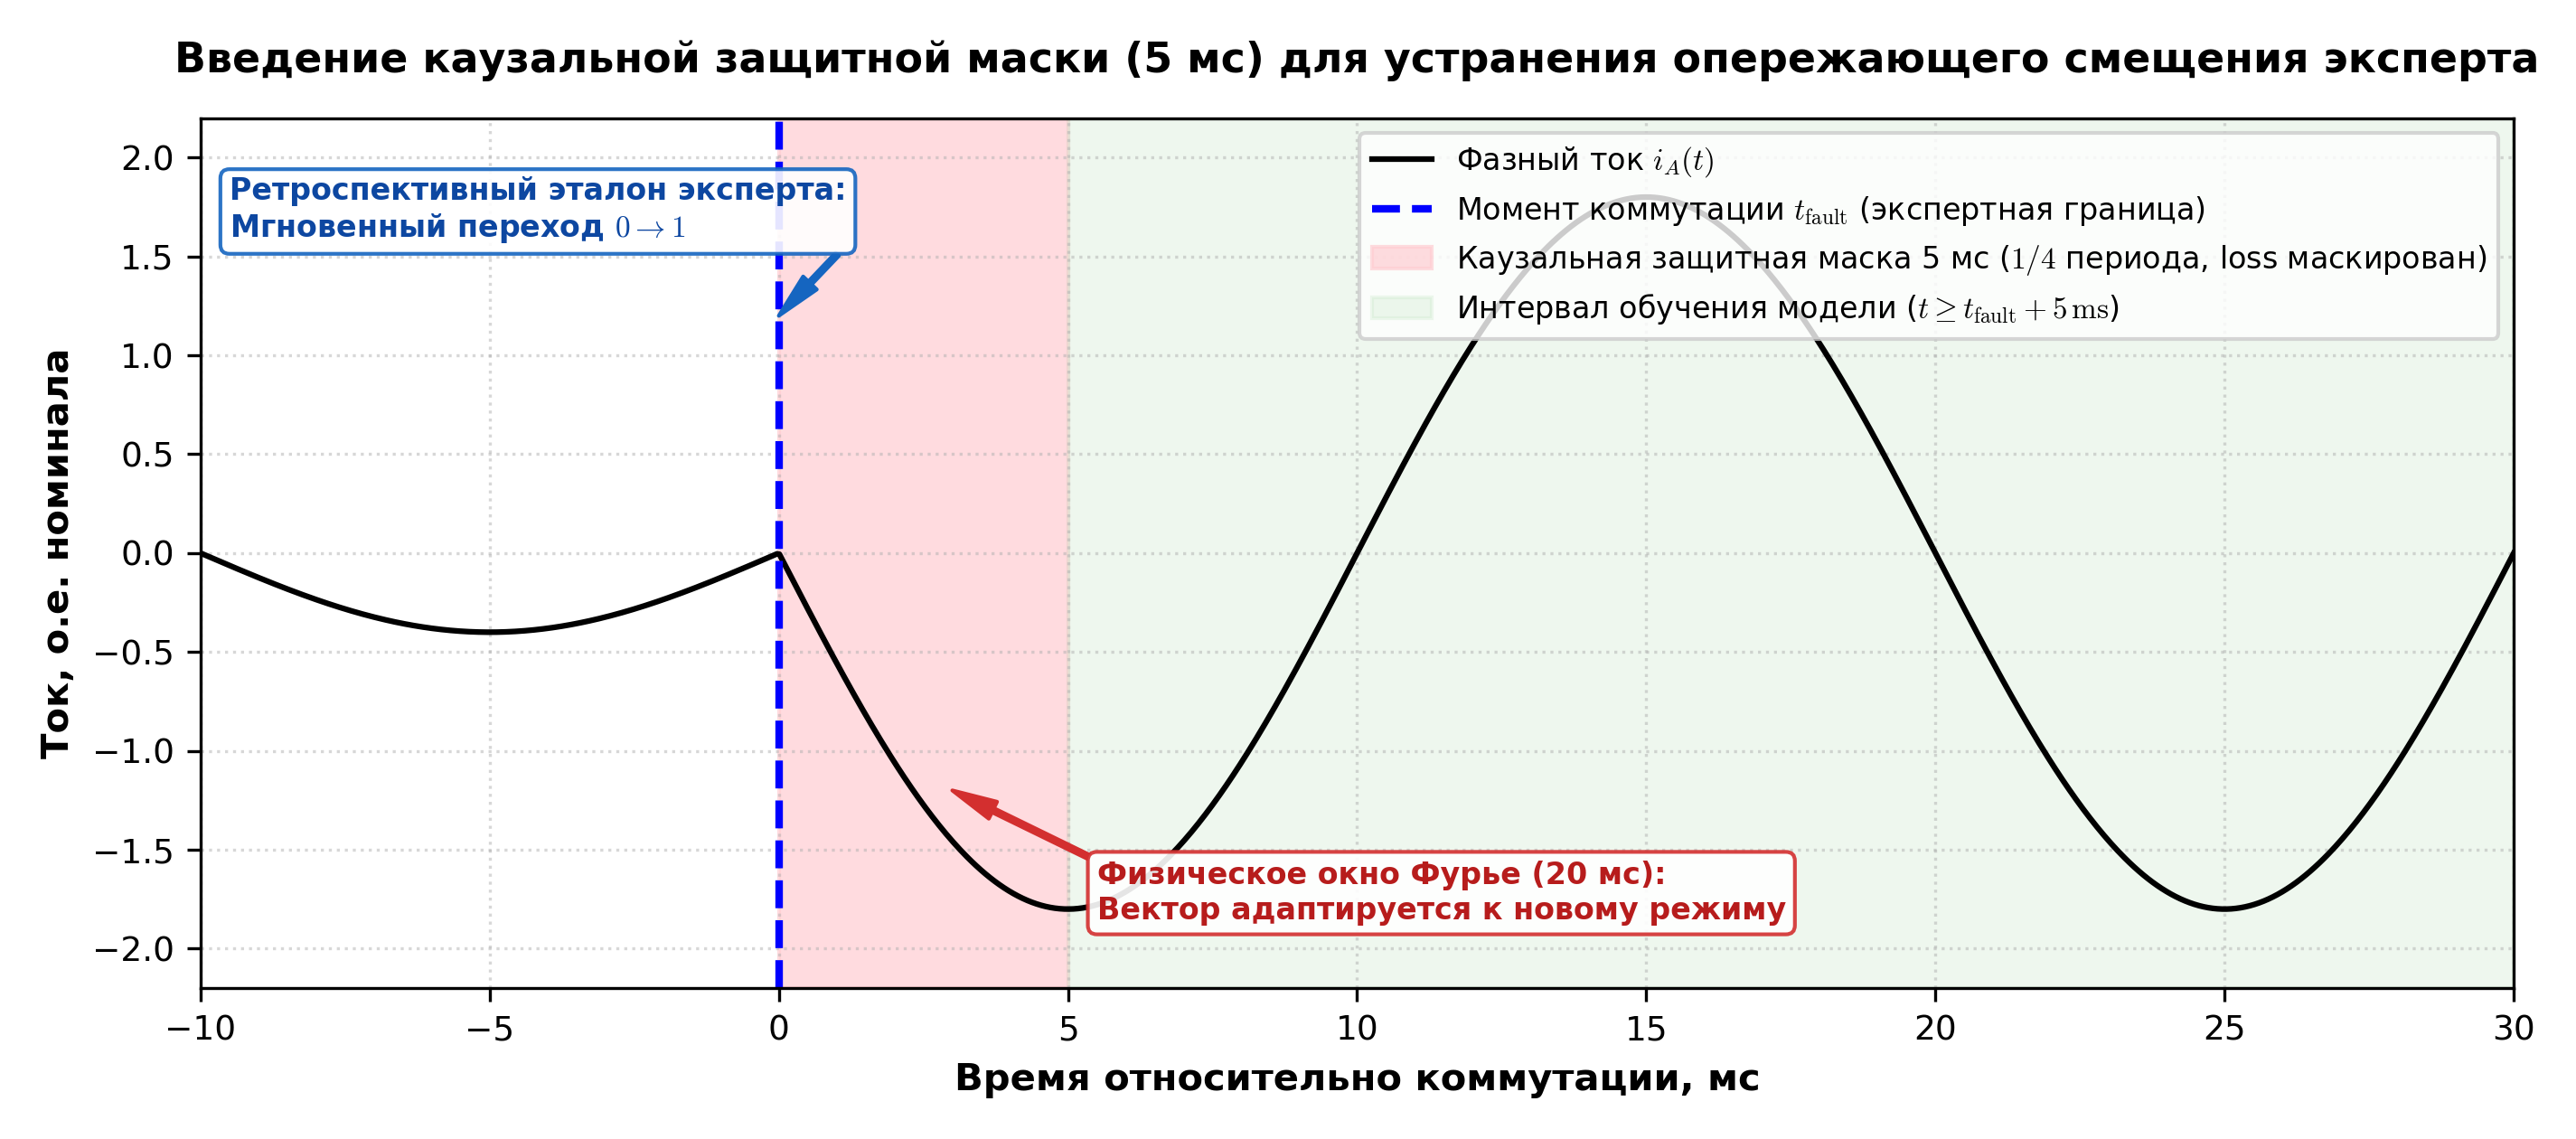
\includegraphics[width=\textwidth]{figures/ch05/ch05_causal_mask_article.png}
\caption{Выделение переходного интервала после экспертной
границы для обучения по уже доступной предыстории}
\label{fig:ch5_causal_mask}
\end{figure}
\figurereview{Исходный рисунок 8 статьи. Сигнал условный.
Сократить заголовок, заменить loss на ошибку обучения.
Зелёное поле не означает, что до него измерительный орган
физически не может выдать правильное решение.}

(Примечание автора: Договориться агентам самим.)


При проверке быстродействия этот интервал сохраняется
и оценивается отдельно. Иначе исключение трудных
границ могло бы скрыть именно те ошибки,
ради которых совершенствуется измерительный орган.
Также отдельно учитывается начальное накопление
данных после начала регистрации.
